% ---------
%  Compile with "pdflatex hw0".
% --------
%!TEX TS-program = pdflatex
%!TEX encoding = UTF-8 Unicode

\documentclass[11pt]{article}
\usepackage{jeffe, handout, graphicx, fancyvrb}
\usepackage{tikz, tikz-qtree}				  % Trees
\usepackage{color}				% Coloring
\usepackage{amsmath}			% Math multilining
\usepackage[utf8]{inputenc}		% Allow some non-ASCII Unicode in source

% =========================================================
%   Define common stuff for solution headers
% =========================================================
\Class{CS 438}
\Semester{Spring 2014}
\Authors{1}
\AuthorOne{Timur Reziapov}{reziapo1}
% =========================================================
\begin{document}

% ---------------------------------------------------------
\HomeworkHeader{6}
\begin{enumerate}[1.]
\item % Problem 1
  \begin{enumerate}[(a)]
  \item \textbf { Challenges of Earth-Mars Slow Start TCP: }

  Starting from a Congestion Window of size 1 is going to be very noticeable because of the much larger delay time. Also the overlall number of RTTs to send a relatively large amount of data will also be much more sensitive in higher numbers. To fix this, it may be more effective to start sending packets with more optimist and a larged Congestion Window. Having a large starting Congestion Window makes the network more vulnerable to congestion problems, therefore it may be beneficial to control and administer strict use of the link.
  \item \textbf { DNS }
    \begin{enumerate}[i.]
    \item \textbf { UDP packet loss:}
    If DNS client times out waiting for the response, it will try to contact the server again. Usually, this timeout indicates that the server is down rather than packet loss, and there is no serious problem.
    \item \textbf { UDP packet max length:}
    DNS names have a size limit of 255 bytes, therefore this should never be a problem. Even if it was, we could send long DNS names in multiple packets and combine them on receiver's side, taking a little care.
    \item \textbf { DNS machine with multiple IP addresses?}
    This is possible. A machine may have multiple ethernet cards, it may be on multiple networks and will need multiple IP addresses.
    \item \textbf { Computer with two DNS names in different top-level domains?}
    This is also possible. Consider www.example.com and www.example.ny.us, both DNS names could have the same IP address. Entires with a com and country-specific domain are possible and quite commmon.
    \end{enumerate} 
  \item \textbf { Wirless node interference: }
  Suppose there are three nodes in the network: A, B and C. B is in range of both A and C, that is the intersection of their ranges, but A and C are separated by a distance greater than either's transmission range and they aren't aware of each other. Now, if A starts sending signals, they will collide with signals from C.

  \item \textbf { Collision detection in wireless networks: }
  Wireless devices cannot 'talk' and 'listen' at the same time, which is a way for Ethernet to detect collisions. Therefore collision detection in wireless networks is extremely difficult, if not impossible and wireless devices employ collision avoidance techniques.
  \end{enumerate}

\newpage
 \item % Problem 2
 \textbf { Longest prefix match using Trie: }
 	\begin{enumerate}[(a)]
 	\item \textbf { Trie Construction: }

    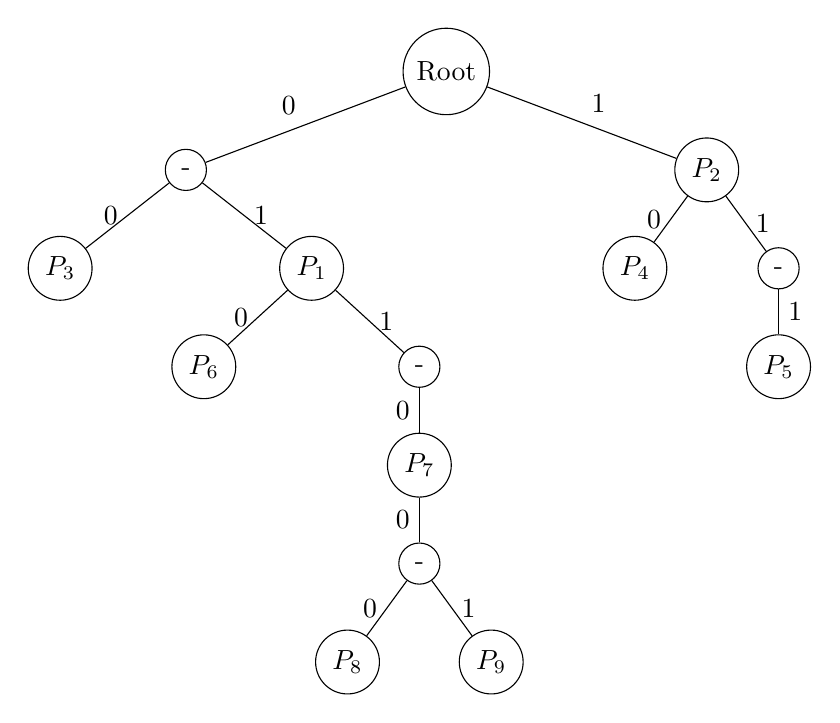
\begin{tikzpicture}[every tree node/.style={draw,circle},
       level distance=1.25cm,sibling distance=1cm,
       edge from parent path={(\tikzparentnode) -- (\tikzchildnode)}]
    \Tree
    [.Root
      \edge node[auto=right] {$0$};
      [.- 
       \edge node[midway,left] {$0$};
       [.$P_3$ ]
       \edge node[midway,right] {$1$};
       [.$P_1$ 
        \edge node[midway,left] {$0$};
        [.$P_6$ ]
        \edge node[midway,right] {$1$};
        [.-
          \edge node[midway,left] {$0$};
          [.$P_7$ 
            \edge node[midway,left] {$0$};
            [.- 
              \edge node[midway,left] {$0$};
              [.$P_8$ ] 
              \edge node[midway,right] {$1$};
              [.$P_9$ ] 
            ]
          ]
        ]
       ]
      ]
      \edge node[auto=left] {$1$};
      [.$P_2$ 
        \edge node[midway,left] {$0$};
        [.$P_4$ ]
        \edge node[midway,right] {$1$};
        [.- 
          \edge node[midway,right] {$1$};
          [.$P_5$ ]
        ]
      ]
    ]
    \end{tikzpicture}

 	\item \textbf {Longest match for:}
 		\begin{itemize}
 		\item 101.174.252.14
    $\to$ 01100101.10101110.11111100.00001110 $\to$ $P_9$

 		\item 97.128.255.17
    $\to$ 01100001.10000000.11111111.00010001 $\to$ $P_8$

 		\item 255.255.255.255
    $\to$ 11111111.11111111.11111111.11111111 $\to$ $P_5$
 		\end{itemize}
 	\end{enumerate}

 \item % Problem 3
 \textbf { TCP RTT Estimation: }
 	\begin{enumerate}[(a)]
 	\item \textbf{ 
    \boldmath{$\alpha = 0.8$, $SRTT(0) = 3$, all measured $RTT$ values = 1 second, no packet loss:}
  } \\
  \begin{align*}
    SRTT(k+1) &= 0.8 \times SRTT(k) + 0.2 \\
      &= 0.8 \times (0.8 \times SRTT(k-1) + 0.2) + 0.2 \\
    \text{with SRTT(0) = 3, } & \text{the recurrence becomes:}\\ 
    SRTT(k) &= 2 * 0.8^k + 1 \\
    SRTT(19) &= 2 * 0.8^{19} + 1 \\
      &= 1.028823 \text{ seconds}
  \end{align*}
 	\item \textbf{
    \boldmath{$SRTT(0) = 1$, $RTT$ values = 3, no packet loss}
  } \\
  \begin{align*}
    SRTT(k+1) &= 0.8 \times SRTT(k) + 0.6 \\
    &= 0.8 \times (0.8 \times SRTT(k-1) + 0.6) + 0.6 \\
    \text{with SRTT(0) = 1, } & \text{the recurrence becomes:}\\ 
    SRTT(k) &= (1-3) * 0.8^k + 3 \\
    SRTT(19) &= -2 * 0.8^{19} + 3 \\
    &= 2.971177 \text{ seconds}
  \end{align*}
 	\end{enumerate}

 \newpage
 \item % Problem 4
 \textbf { Congestion Control: }
 	\begin{enumerate}[(a)]
 	\item \textbf{
    \boldmath{ $RTT$ delay = 95 ms, $Bandwidth$ = 2 Gbps, $Segment$ $Size$ = 576 octets:}
  } \\
  Windows Size in bits: $95\ ms \times 2\ Gbps = 190 * 10^6\ bits$\\
  $Segment Size = 576 * 8 = 4608\ bits$ \\
  Window Size in packets: 
  \begin{align*}
    \left\lceil\frac{190*10^6}{4608}\right\rceil = 41233\ packets\\
  \end{align*} 
  Congestion window will halve to 20617 packets after timeout. TCP will use slow start to reach  the congestion threshold, in exponential increase to a window size of $2^{15} = 32768$ (the next bigger power of 2), which will take 15 RTT. From then on, we get to the full window size using additive increase, which will take $41233 - 32768 = 8465$ RTT. The total time to reach full Window Size after timeout: 
  \begin{align*}
    (15 + 8465) \times RTT = 8480 \times 95\ ms = 805.6\ s
  \end{align*}

 	\item \textbf{ 
    \boldmath{Repeat for $Segment Size$ = 16 Kbytes}
  }\\
  $Segment Size = 16 * 1024 * 8 = 131072\ bits$ \\
  Window Size in packets: 
  \begin{align*}
    \left\lceil\frac{190*10^6}{131072}\right\rceil = 1450\ packets\\
  \end{align*} 
  Congestion window will halve to 725 packets after timeout. TCP will use slow start to reach  the congestion threshold, in exponential increase to a window size of $2^{10} = 1024$ (the next bigger power of 2), which will take 10 RTT. From then on, we get to the full window size using additive increase, which will take $1450 - 1024 = 426$ RTT. The total time to reach full Window Size after timeout: 
  \begin{align*}
    (10 + 426) \times RTT = 436 \times 95\ ms = 41.42\ s
  \end{align*}
 	\end{enumerate}
\end{enumerate}
\end{document}
